%%%%%%%%%%%%%%%%%%%%%%%%%%%%%%%%%%%%%%%%%%%%%%%%%%%%%%%%%%%%%%%%%%%%%%%%%%%%%%%%
%2345678901234567890123456789012345678901234567890123456789012345678901234567890
%        1         2         3         4         5         6         7         8

\documentclass[letterpaper, 10 pt, conference]{ieeeconf}  % Comment this line out
                                                          % if you need a4paper
%\documentclass[a4paper, 10pt, conference]{ieeeconf}      % Use this line for a4
                                                          % paper

\IEEEoverridecommandlockouts                              % This command is only
                                                          % needed if you want to
                                                          % use the \thanks command
\overrideIEEEmargins
% See the \addtolength command later in the file to balance the column lengths
% on the last page of the document



% The following packages can be found on http:\\www.ctan.org
\usepackage{amsmath} % assumes amsmath package installed
\usepackage{amssymb}  % assumes amsmath package installed
\usepackage{tikz} % assumes tikz package installed
\usepackage{subfig} % assumes subfig package installed
\title{\LARGE \bf
Inferring Network Topology from Chaotic Time Series
}

\author{Parker King-Fournier \\
		parker.king-fournier "at" gmail.com}

\begin{document}

\maketitle
\thispagestyle{empty}
\pagestyle{empty}

%%%%%%%%%%%%%%%%%%%%%%%%%%%%%%%%%%%%%%%%%%%%%%%%%%%%%%%%%%%%%%%%%%%%%%%%%%%%%%%%
\begin{abstract}
Significant interest has been shown in the ability of ecologic networks to generate chaotic dynamics: it has been shown that even simple ecologic models can generate  dynamics that neither reach an equilibrium nor a stable limit cycle, but oscillate around a strange attractor. The resulting chaos has proved challenging to analyze due to its sensitivity to initial conditions and lack of homogeneity. In this paper three machine learning classification models are used to infer the topology of ecologic networks that were found to produce chaotic dynamics. The classification accuracy of a Deep Neural Network (DNN), Convolutional Neural Network (CNN) and Convolutional - Long Short Term Memory Network (CNN-LSTM) are compared and a positive correlation between model complexity and classification accuracy was found with the  CNN-LSTM performing on average best, the CNN second best, and the DNN worst. 
\end{abstract}
\begin{keywords}
chaos theory, chaotic attractors, convolutional neural networks, deep neural networks, dynamical systems, ecology, food webs, long short term memory, machine learning, network topology, time series, sequence classification 
\end{keywords}


%%%%%%%%%%%%%%%%%%%%%%%%%%%%%%%%%%%%%%%%%%%%%%%%%%%%%%%%%%%%%%%%%%%%%%%%%%%%%%%%
\section{INTRODUCTION}
	Chaos Theory has provided explanations to the seemingly unpredictable nature of many systems in our universe. Characterized by their sensitivity to initial conditions, chaotic systems yield drastically different results from minute changes in starting conditions, making them difficult to analyze using traditional methods. Systems both natural and man-made have been shown to exhibit chaotic behavior. In nature chaos is found often in the flow of liquid and gases. The famous Lorenz system, a simplified model of atmospheric weather patterns, shows chaotic dynamics for certain parameter settings (Lorenz, 1993). Man-made systems, such as the double pendulum and logistic map have helped further the understanding of chaos and its applications.

	The study of chaos has been widely successful to the study of time series (Liu, 2010), showing how markets, particles' positions, or populations may change over time. In the field of ecology the well known Lynx-Hare Cycle has shown that population dynamics of species may be governed by chaos (Maquet, 2007). The application of chaos theory to the study of population dynamics has continued and, has been successful in describing the populations of species contained within certain food web structures (Klebanoff, 1994).

	Due to the deterministic nature of chaos, a chaotic system can be successfully predicted if the underlying processes of the system are known. Without this information however, the prediction and overall analysis of these systems is difficult due to the erratic characteristics present. Recent developments in the field of Machine Learning have increased the ability to predict and characterize chaotic systems. Because these algorithms have the ability to learn complex functions, extract features from data and generalize well, Machine Learning is being used to explore chaotic systems in both academia and industry. 
    
	Despite the rising popularity of Machine Learning, its use in the field of ecology has been slow growing. The presence of chaos in ecology and the ability for Machine Learning to understand complicated dynamics exposes one use of Machine Learning in ecology and is the main motivation for the following report.
    
	Below is a detailed description of one such application of the power Machine Learning in the analysis of chaotic dynamics originating from ecological systems. First, a dataset of population data is created from food web models which are known to show chaos. Each point in this dataset contains a chaotic population time series, and the topology of the food web that generated the time series. This data set is then split into multiple smaller datasets to allow comparison between subsets of the data. 
    
	The datasets created are then used to train three Machine Learning algorithms with the aim of classifying the population time series by the food web topology that governed the dynamics. The results are interpreted with respect to their importance in the fields of ecology and machine learning, and improvements to the models and datasets are discussed so that further research may be well directed.  

%%%%%%%%%%%%%%%%%%%%%%%%%%%%%%%%%%%%%%%%%%%%%%%%%%%%%%%%%%%%%%%%%%%%%%%%%%%%%%%%
\section{RELATED WORK}
	As stated above, the presence of chaos in ecologic systems has been the focus of much previous research. In \textit{"Do Strange Attractors Govern Ecological Systems?"} Schaffer and Kot explored the presence of chaotic dynamics in theoretical models as well as real world data (Schaffer \& Kot, 1985). The chaos was visualized revealing attractors along which various natural systems travel. Schaffer and Kot challenged the existing understanding of natural systems, speculating that (then) current linear models may severely misrepresent the complexity of nature. 
    
	Furthermore, the authors speculated that natural systems may be entirely nonlinear saying, "Our own opinion is that what passes for fundamental concepts in ecology is as mist before the fury of the storm-in this case, a full, nonlinear storm" (Schaffer \& Kot, 1985). Although significant time has passed since publication, this work provides important theoretic and empirical evidence that chaos is present in natural systems. 
    
	It is well established that food webs can generate chaotic dynamics for certain parameter settings. In 1994 Aaron Klebanoff and Alan Hastings showed chaotic dynamics in their paper titled \textit{"Chaos in one-predator, two-prey models: General results from bifurcation theory"} (Klenaboff \& Hastings, 1994). Their work showed that a relatively simple system can produce extremely erratic results, and again secured the place of Chaos Theory in ecology. 
  
	The prospect of inferring network topology from data is an important problem in ecology. Previous work includes the inference of topology in spatial networks (Barthelemy et al., 2010), as well as the inference of topology in networks describing species interaction (Vera-Licona \&  Laubenbacher, 2008). 
  
	In \textit{"Inferring topology from dynamics in spatial networks"}, Gilarranz et al. attempted to discern the degree to which the dynamical patterns reveal underlying dispersal pathways. Their attempt was unsuccessful but their apparent failure proved to be helpful by showing that further constraints must be made in order to make the inference more manageable for our current technologies. This was a main factor in the decision to restrict the number of classes present in the datasets created for this report. 

	The classification of population data into different generating topologies falls under the larger task of sequence classification. In the Machine Learning community sequence classification has been used in a variety of applications, from medical diagnosis to human-robot differentiation (Dietterich, 2002). Of particular interest is the recent work on the performance of Deep Learning methods, specifically Long Short Term Memory (LSTMs) Networks, in sequence classification. In 2005 Alex Graves and Jurgen Schmidhuber found that LSTM Networks outperformed traditional Recurrent Neural Networks (RNNs) and Multilayer Perceptrons (MLPs) in speech processing. While speech processing may seem a long way from ecological networks, the performance of the networks in the task of sequence classification inspired some of the architectures used below. 

%%%%%%%%%%%%%%%%%%%%%%%%%%%%%%%%%%%%%%%%%%%%%%%%%%%%%%%%%%%%%%%%%%%%%%%%%%%%%%%%
\section{PROBLEM DESCRIPTION}
\begin{figure}
  \centering
  \subfloat[A trajectory in the ZYX phase space showing the presence of chaos.]{\label{ref_label1}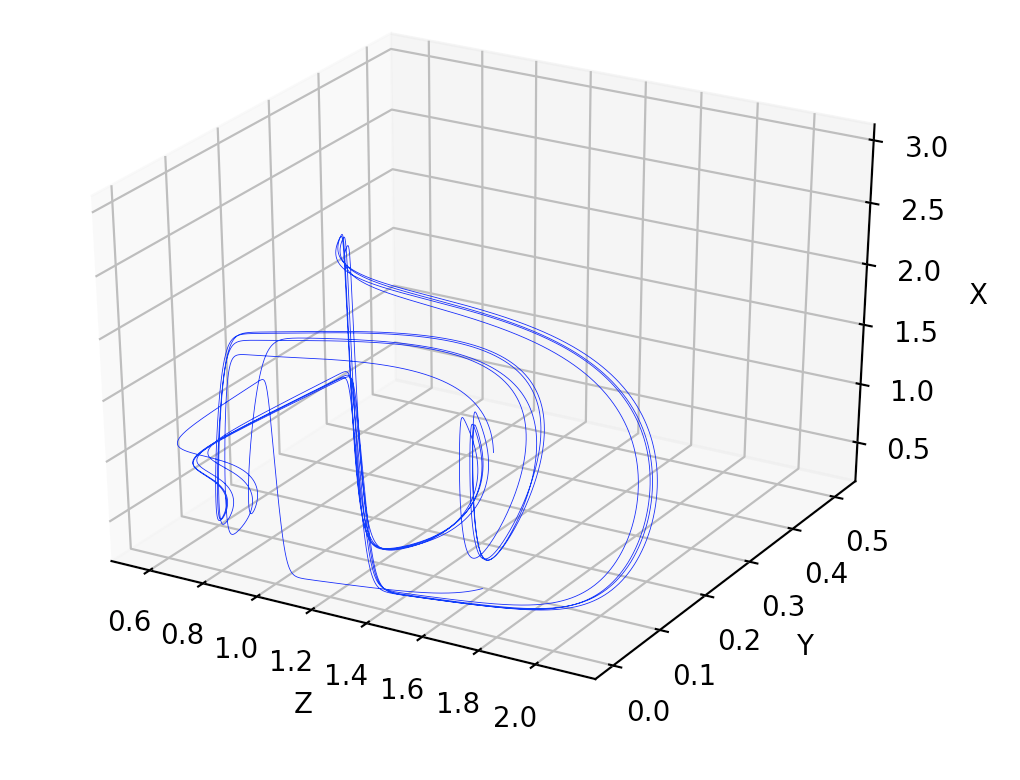
\includegraphics[width=0.5\textwidth]{zyx.png}}\\
  \subfloat[A trajectory in the YXC phase space showing the presence of chaos.]{\label{ref_label2}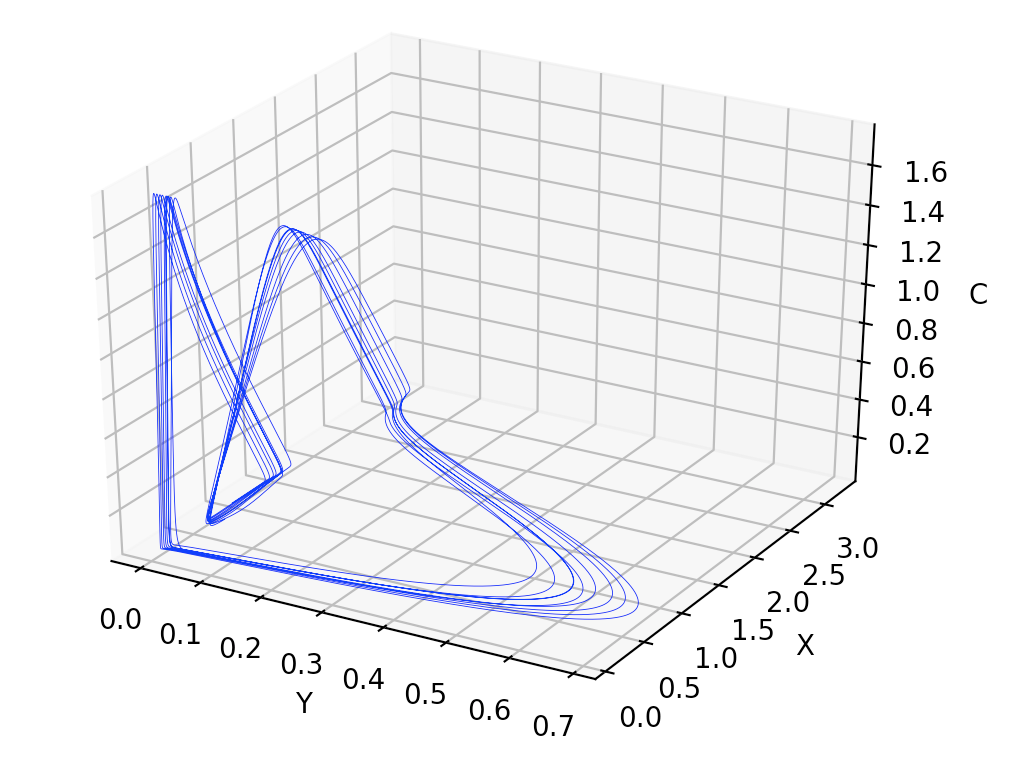
\includegraphics[width=0.5\textwidth]{yxc.png}}\\
  \subfloat[A trajectory in the XCP phase space showing the presence of chaos.]{\label{ref_label3}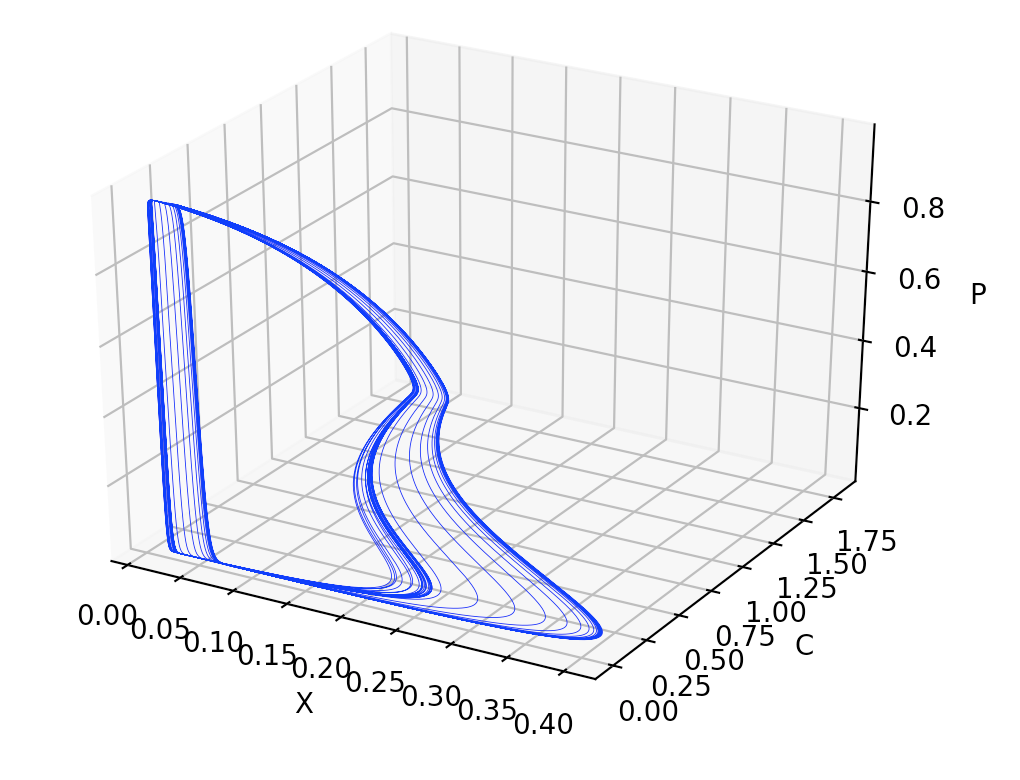
\includegraphics[width=0.5\textwidth]{xcp.png}}\\
  \caption{\label{ref_label_overall}Phase space trajectories for a 5 species chain. Z represents the apex predator of the chain, Y is predated by Z, X is predated by Y, C is predated by X and P is predated by C. Trajectories show the presence of chaos in the models used to generate the data sets.}
\end{figure}

	The goal of the research presented was to attempt to infer characteristics of the underlying food web topology of a system given a population single time series. Originally the aim was to generate the underlying topology after observing a time series, however it became clear early on that this approach was too broad. To narrow the scope the number of topologies considered was limited to eight different network structures. 
    
    Using preexisting ecologic models these topologies were used to generate chaotic time series that were stored in a data set containing points of the form \textit{(X , Y)}, where \textit{X} is the time series of a single species and \textit{Y} is the food web topology that generated \textit{X}.
    
    To further understand the difference between topologies, this original data set was relabeled and stored into a new data set of the form \textit{(X , Y')}, where \textit{X} is the time series of a single species and \textit{Y} is the number of species in the topology that generated \textit{X}. Additionally, a data set was created for each class \textit{y} $\epsilon$ \textit{Y'}. These sets were stored in the same format as the previously mentioned data sets. A more rigorous description of the data sets is below. 
    
    After creating the datasets, three classification algorithms were trained on each data set, and the highest accuracy for each were recorded. The classification algorithms used represented a variety of approaches to classification: specifically these algorithms were a Deep Neural Network (DNN), Convolutional Neural Network (CNN), and a Convolutional - Long Short Term Memory Network (CNN-LSTM). 
    
\subsection{Ecological Models}
\begin{table}
\tikzstyle{every node}=[circle, draw, fill=black,
                        inner sep=0pt, minimum width=1pt]
\caption{Food Web Topologies}
\setlength{\tabcolsep}{5mm} % separator between columns
\def\arraystretch{1.25} % vertical stretch factor
\centering

  \begin{tabular}{|c|c|c|}
	\hline
    & A & B \\
    \hline
    1 & 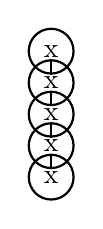
\begin{tikzpicture}[thick,scale=0.8]
   		\node at (0,-0) [circle,draw] (a) {x};
        \node at (0,-0.5) [circle,draw] (b) {x};
        \node at (0,-1) [circle,draw] (c) {x};
        \node at (0,-1.5) [circle,draw] (d) {x};
        \node at (0,-2) [circle,draw] (e) {x};
        \draw (a) -- (b) -- (c) -- (d) -- (e);
    \end{tikzpicture} &
    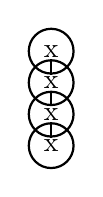
\begin{tikzpicture}[thick,scale=0.8]
   		\node at (0,0) [circle,draw] (a) {x};
        \node at (0,-0.5) [circle,draw] (b) {x};
        \node at (0,-1) [circle,draw] (c) {x};
        \node at (0,-1.5) [circle,draw] (d) {x};
        \draw (a) -- (b) -- (c) -- (d);
    \end{tikzpicture} \\  
    \hline
    
    2 & 
    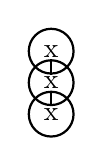
\begin{tikzpicture}[thick,scale=0.8]
   		\node at (0,0) [circle,draw] (a) {x};
        \node at (0,-0.5) [circle,draw] (b) {x};
        \node at (0,-1) [circle,draw] (c) {x};
        \draw (a) -- (b) -- (c);
    \end{tikzpicture} &
    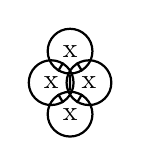
\begin{tikzpicture}[thick,scale=0.8]
   		\node at (0,0) [circle,draw] (a) {x};
        \node at (-0.3,-0.5) [circle,draw] (b1) {x};
        \node at (0.3,-0.5) [circle,draw] (b2) {x};
        \node at (0,-1) [circle,draw] (c) {x};
        \draw (a) -- (b1) -- (c) (a) -- (c) (a) -- (b2) -- (c);
    \end{tikzpicture}  \\ 
    \hline
    
    3 & 
    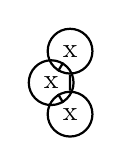
\begin{tikzpicture}[thick,scale=0.8]
   		\node at (0,0) [circle,draw] (a) {x};
        \node at (-0.3,-0.5) [circle,draw] (b) {x};
        \node at (0,-1) [circle,draw] (c) {x};
        \draw (a) -- (b) -- (c) (a) -- (c);
    \end{tikzpicture}   &
    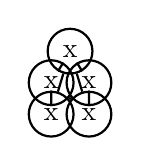
\begin{tikzpicture}[thick,scale=0.8]
   		\node at (0,0) [circle,draw] (a) {x};
       	\node at (-0.3,-0.5) [circle,draw] (b1) {x};
        \node at (0.3,-0.5) [circle,draw] (b2) {x};
        \node at (-0.3,-1) [circle,draw] (c1) {x};
        \node at (0.3,-1) [circle,draw] (c2) {x};
        \draw (a) -- (b1) -- (c1) (a) -- (b2) -- (c2) (b1) -- (c2) (b2) -- (c1) (a) -- (c1) (a) -- (c2);
    \end{tikzpicture} \\ 
    \hline
   
   4 & 
   	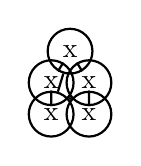
\begin{tikzpicture}[thick,scale=0.8]
   		\node at (0,0) [circle,draw] (a) {x};
       	\node at (-0.3,-0.5) [circle,draw] (b1) {x};
        \node at (0.3,-0.5) [circle,draw] (b2) {x};
        \node at (-0.3,-1) [circle,draw] (c1) {x};
        \node at (0.3,-1) [circle,draw] (c2) {x};
        \draw (a) -- (b1) -- (c1) (a) -- (b2) -- (c2) (b1) -- (c2) (b2) -- (c1) (a) -- (c1);
    \end{tikzpicture}   &
    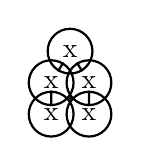
\begin{tikzpicture}[thick,scale=0.8]
   		\node at (0,0) [circle,draw] (a) {x};
       	\node at (-0.3,-0.5) [circle,draw] (b1) {x};
        \node at (0.3,-0.5) [circle,draw] (b2) {x};
        \node at (-0.3,-1) [circle,draw] (c1) {x};
        \node at (0.3,-1) [circle,draw] (c2) {x};
        \draw (a) -- (b1) -- (c1) (a) -- (b2) -- (c2) (b1) -- (c2) (b2) -- (c1);
    \end{tikzpicture} \\ 

   \hline
  \end{tabular}
\end{table}

	For the creation of the data sets used the models described in by Fussman and Heber in \textit{"Food web complexity and chaotic population dynamics"} were adopted (Fussman \& Heber, 2002). To limit the number of classes, only the eight topologies demonstrating the highest amount of chaos were used (Table 1). While evaluating these models all parameter values were kept consistent to those used by Fussman and Heber in order to ensure that the time series generated would be similarly consistent. For the convenience of the reader the general form of the differential equations describing the food web in Fig. 2 are presented:
    
\begin{multline}
	\frac{dP_i}{dt} =
    P_i\Bigg{[} 
    	r_i(1-\frac{P_i}{K_i}) - 
    	\frac{a_{P_i}^{C_1}C_1}{1 + b_{P_1}^{C_1}P_1 + b_{P_2}^{C_1}P_2 + b_{P_2}^{C_1}P_3} \\
   		-  \frac{a_{P_i}^{C_2}C_2}{1 + b_{P_1}^{C_2}P_1 + b_{P_2}^{C_2}P_2 + b_{P_2}^{C_2}P_3} \\
    	- \frac{a_{P_i}^{X}X}{1 + b_{P_1}^{X}P_1 + b_{P_2}^{X}P_2 + b_{P_3}^{X}P_3 + b_{C_1}^{X}C_1 + b_{C_2}^{X}C_2}
	\Bigg{]}, \\
    i = 1,2,3
\end{multline}

\begin{multline}
	\frac{dC_i}{dt} =
   	C_i\Bigg{[} 
    	\frac{a_{P_1}^{C_i}P_1 + a_{P_2}^{C_i}P_2 + a_{P_2}^{C_i}P_3}{1 + b_{P_1}^{C_i}P_1 + b_{P_2}^{C_i}P_2 + b_{P_2}^{C_i}P_3} \\
        - \frac{a_{C_i}^{X}X}{1 + b_{P_1}^{X}P_1 + b_{P_2}^{X}P_2 + b_{P_3}^{X}P_3 + b_{C_1}^{X}C_1 + b_{C_2}^{X}C_2} - d_{C_i}
    \Bigg{]} \\
    i = 1,2
\end{multline}

\begin{multline}
	\frac{dX}{dt} =
   		X\Bigg{[} 
        \frac{{a_{P_1}^{X}P_1 + a_{P_2}^{X}P_2 + a_{P_3}^{X}P_3 + a_{C_1}^{X}C_1 + a_{C_2}^{X}C_2}}{{1 + b_{P_1}^{X}P_1 + b_{P_2}^{X}P_2 + b_{P_3}^{X}P_3 + b_{C_1}^{X}C_1 + b_{C_2}^{X}C_2}} \\ 
        - \frac{a_X^YY}{1 + b_X^YX} - d_X
        \Bigg{]}
\end{multline}

\begin{equation}
	\frac{dY}{dt} =
    Y\Bigg{[}
    	\frac{a_X^YY}{1 + b_X^YX} - \frac{a_Y^ZZ}{1 + b_Y^ZY} - d_Y
    \Bigg{]}
\end{equation}

\begin{equation}
	\frac{dZ}{dt} =
    Z\Bigg{[}
    	\frac{a_Y^ZY}{1 + b_Y^ZY}  - d_Z
    \Bigg{]}
\end{equation}


The food web topologies and differential equations shown were found to exhibit chaotic dynamics for certain parameter settings. Figure 1 shows different visualizations of one phase space trajectory of the most chaotic network topology, the chain of length 5. 

\subsection{Datasets}
A total of 5 data sets were created. Of these five data sets four are subsets of the original data set, denoted \textit{D}. The relationship of these data sets to one another is shown in Figure 2. \textit{D} was created by holding all parameter values constant except for the mortality rates \textit{d\textsubscript{C\textsubscript{i}}}, \textit{d\textsubscript{Y}}, \textit{d\textsubscript{Y}}, and \textit{d\textsubscript{Z}}. The n-dimensional space of mortality rates was traversed (Table 2), evaluating the differential equations (1) through (5) 200,000 time steps for each parameter combination, and omitting the first 50,232 time steps to remove any trajectories not on an attractor. Following Fussman and Heber (Fussman \& Heber, 2002), the resulting time series of length 149769, denoted \textit{x}, was recorded only if every species in the network "survived". This was carried out by only recording time series for which all species populations were greater than the threshold value $\varepsilon$ = 10\textsuperscript{-9} at time \textit{t} = 200,000. 

\textit{D} thus has the form \textit{(\textbf{X}, \textbf{Y})}, where \textit{\textbf{X}} is a vector of time series and \textit{\textbf{Y}} is a vector of labels such that each \textit{x} $\epsilon$ \textit{\textbf{X}} was generated by evaluating equations (1) through (5) corresponding to topology \textit{y} $\epsilon$ \textit{\textbf{Y}}. From \textit{D}, four data sets were created. The first, \textit{D\textsubscript{N}}, is of the form \textit{(\textbf{X}\textsubscript{N}, \textbf{Y}\textsubscript{N})}, where \textit{\textbf{X}\textsubscript{N}} = \textit{\textbf{X}} and each \textit{\textbf{Y}\textsubscript{Ni}} $\epsilon$ \textit{\textbf{Y}\textsubscript{N}} is a class corresponding to the number of species in topology \textit{y} $\epsilon$ \textit{\textbf{Y}}. From \textit{D\textsubscript{N}} three data sets,  \textit{D\textsubscript{3}}, \textit{D\textsubscript{4}} and \textit{D\textsubscript{5}}, were created: for each \textit{D\textsubscript{i}}, \textit{i} = 1, 2, 3, data points \textit{(x, y)} $\epsilon$ \textit{(\textbf{X}, \textbf{Y})} were recorded if \textit{y} was a topology with \textit{i} species. 

	These five data sets can be understood as a tree, shown in Figure 1. \textit{D} is used to determine which of the eight topologies \textit{y} $\epsilon$ \textit{\textbf{Y}} generated a given time series \textit{x} $\epsilon$ \textit{\textbf{X}}. Set \textit{D\textsubscript{N}} reduces the number of classes by only distinguishing each time series by the number of species in the generating network. Once \textit{D\textsubscript{N}} is used to narrow down possible topologies \textit{D\textsubscript{3}}, \textit{D\textsubscript{4}} and \textit{D\textsubscript{5}} can be used to differentiate between topologies with the same number of species. 
    
\begin{figure}
	\centering
	\tikzstyle{every node}=[circle, draw, fill=gray,
                        inner sep=0pt, minimum width=18pt]
    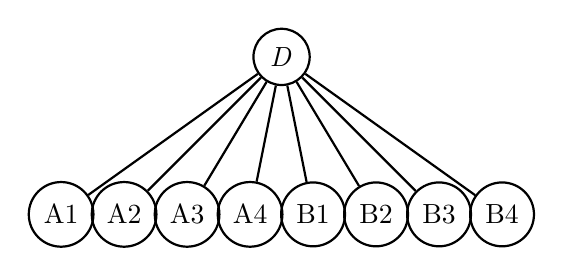
\begin{tikzpicture}[thick,scale=0.8]
   		\node at (0.0,1) [circle,draw] (a) {\textit{D}};
        \node at (-3.5,-1.5) [circle,draw] (b) {A1};
        \node at (-2.5,-1.5) [circle,draw] (c) {A2};
        \node at (-1.5,-1.5) [circle,draw] (d) {A3};
        \node at (-0.5,-1.5) [circle,draw] (e) {A4};
        \node at (0.5,-1.5) [circle,draw] (f) {B1};
        \node at (1.5,-1.5) [circle,draw] (g) {B2};
        \node at (2.5,-1.5) [circle,draw] (h) {B3};
        \node at (3.5,-1.5) [circle,draw] (i) {B4};
        \draw (a) -- (b) (a) -- (c) (a) -- (d) (a) -- (e) (a) -- (f) (a) -- (g) (a) -- (h) (a) -- (i);
    \end{tikzpicture}
\end{figure}    
    
\begin{figure}
	\centering
	\tikzstyle{every node}=[circle, draw, fill=gray,
                        inner sep=0pt, minimum width=18pt]
    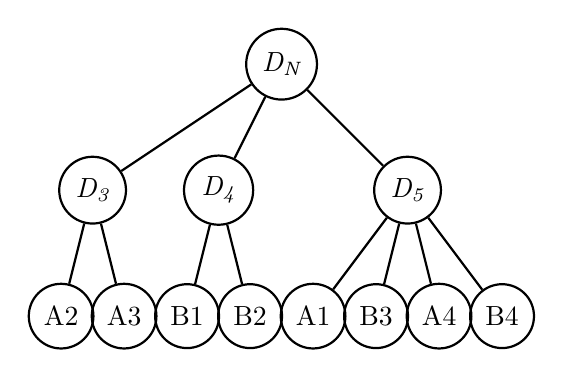
\begin{tikzpicture}[thick,scale=0.8]
    	\node at (0.0,1) [circle,draw] (a) {\textit{D\textsubscript{N}}};
        
        \node at (-3,-1) [circle,draw] (b) {\textit{D\textsubscript{3}}};
        \node at (-1,-1) [circle,draw] (c) {\textit{D\textsubscript{4}}};
        \node at (2,-1) [circle,draw] (d) {\textit{D\textsubscript{5}}};
        
        \node at (-3.5,-3) [circle,draw] (e) {A2};
        \node at (-2.5,-3) [circle,draw] (f) {A3};
        \node at (-1.5,-3) [circle,draw] (g) {B1};
        \node at (-0.5,-3) [circle,draw] (h) {B2};
        \node at (0.5,-3) [circle,draw] (i) {A1};
        \node at (1.5,-3) [circle,draw] (j) {B3};
        \node at (2.5,-3) [circle,draw] (k) {A4};
        \node at (3.5,-3) [circle,draw] (l) {B4};
        \draw (a) -- (b) (a) -- (c) (a) -- (d) (b) -- (e) (b) -- (f) (c) -- (g) (c) -- (h) (d) -- (i) (d) -- (j) (d) -- (k) (d) -- (l);
        \end{tikzpicture}
        \caption{The partitioning of data into different sets. The top tree shows data set \textit{D} as the root node, with each topology as the leaves. The bottom tree shows the relationship of \textit{D\textsubscript{3}}, \textit{D\textsubscript{4}} and \textit{D\textsubscript{5}} as subsets of \textit{D\textsubscript{N}}, with \textit{D\textsubscript{N}} being the root and each topology as the leaves}
\end{figure}


\begin{table}
\caption{Mortality Rate Parameter Space}
\setlength{\tabcolsep}{5mm} % separator between columns
\def\arraystretch{1.25} % vertical stretch factor
\centering

  \begin{tabular}{|c|c|}
	\hline
    \textbf{Parameter} & \textbf{Range} \\ \hline
    \textit{d\textsubscript{C\textsubscript{i}}}& \lbrack0.01, 1.2\rbrack \\ \hline
	\textit{d\textsubscript{X}}& \lbrack0.01, 0.42\rbrack \\ \hline
    \textit{d\textsubscript{Y}}& \lbrack0.0, 0.14\rbrack \\ \hline
    \textit{d\textsubscript{Z}}& \lbrack0.01, 0.06\rbrack \\ \hline
  \end{tabular}
\end{table}


\subsection{Classification Models}
	To classify the time series data three Machine Learning algorithms were trained and tested on the data sets described above. These algorithms, specifically a DNN, a CNN and a CNN-LSTM, were chosen because of their differences in network complexity, with the DNN being the most simple and the CNN-LSTM being the most complex, and because each possesses strengths and weaknesses in relation to certain types of data. The difference in how each algorithm performs may express some hidden trait of the ecological networks used to generate the data sets. A description of the architecture of each algorithm follows.
    
    The architecture of the DNN is a rather straightforward architecture, and was chosen to act as a pseudo baseline as DNNs are a standard first approach in most Machine Learning applications. The specific architecture featured an input layer of size 149769, followed by five hidden layers of size 50 each, with the output layer having a size equal to the number of classes in data set used. For example, if the DNN were trained and evaluated on \textit{D} the output layer would have size 8 (Fig. 3). To combat overfitting a dropout rate of 0.5 was used while training the network. 
    
    Because the size of the largest data set was still relatively small, containing only 2156 data points, a deep but skinny network architecture was favored due to a greater ability to generalize. A wide but shallow network may have memorized the data rather than computing a useful classification function. 
    
    The next most complex classification model, the CNN, was chosen as a medium complexity model to compare against the DNN. While CNNs are widely known for their use in computer vision and image classification, their ability to extract features from data autonomously has shown them to be useful in many fields (Voulodimos et al., 2018). 
    
    The CNN used utilized one-dimensional convolutions on the input to extract such features. Specifically, the architecture had an input layer of size 149769, followed by 5 hidden convolutional layers, each followed by a max pooling layer, and one fully connected layer wit a dropout rate of 0.5. This was followed by the final layer having again a size equal to the number of classes in the data set used. A complete diagram of the CNN is shown in Figure 4. 
    
    Lastly, the CNN-LSTM was chosen do to its high model complexity. LSTMs are know to excel in learning from sequential data (Graves \& Jurgen Schmidhuber, 2005), and are robust against problems of long term dependency. Because of this, the CNN-LSTM was chosen as the so-called heavy hitter of the classification algorithms. This architecture represents the combination of two pre existing architectures: it uses a series of one-dimensional convolutions which then pass the data into a LSTM layer (Fig. 5) . Finally the data is passed from the LSTM cell to a fully connected layer with a dropout rate of 0.5 and to an output layer similar to those above. 
 
\begin{figure}
	\centering
    {\label{ref_label1}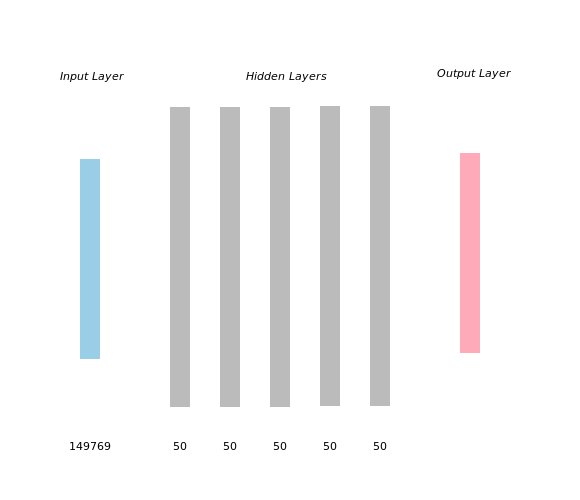
\includegraphics[width=0.5\textwidth]{dnn.png}}
    \caption{\label{ref_label_overall}The network architecture of the Deep Neural Network. The labels along the bottom represent the number of nodes in each layer. The output layer is left without a size as it will always be equal to the number of classes in the data set used to train the DNN.}
\end{figure}
 
\begin{figure}
	\centering
	{\label{ref_label1}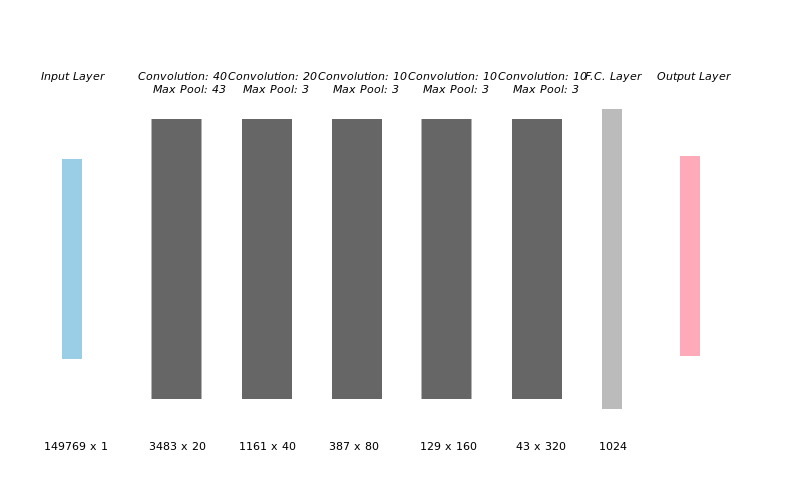
\includegraphics[width=0.5\textwidth]{cnn.png}}
    \caption{\label{ref_label_overall}The network architecture of the Convolutional Neural Network (CNN). The labels along the bottom represent the dimension of each convolutional layer or the number of nodes in a layer. The output layer is left without a size as it will always be equal to the number of classes in the data set used to train the CNN.}
\end{figure} 

\begin{figure}
	\centering
    {\label{ref_label2}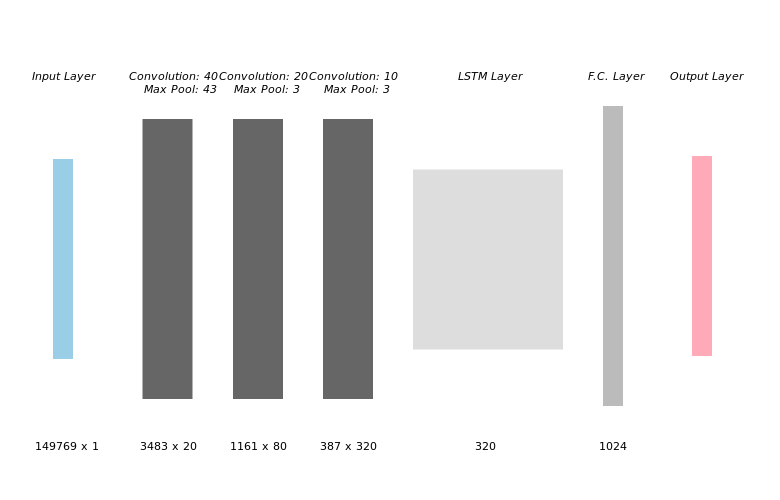
\includegraphics[width=0.5\textwidth]{cnn_lstm.png}}
    \caption{\label{ref_label_overall}The network architecture of the Convolutional Long Short Term Memory Network (CNN-LSTM). The labels along the bottom represent the dimension of each convolutional layer or the number of nodes in a layer. The output layer is left without a size as it will always be equal to the number of classes in the data set used to train the CNN-LSTM.}
\end{figure} 

%%%%%%%%%%%%%%%%%%%%%%%%%%%%%%%%%%%%%%%%%%%%%%%%%%%%%%%%%%%%%%%%%%%%%%%%%%%%%%%%
\section{METHODS}
\subsection{Dataset Creation}
	All data sets constructed using the ecological models above implemented in python. To approximate the integration of equations (1) through (5) the following form was used:
\begin{equation}x_{t+1} = x_{t} + f(x_{t})dt\end{equation}
where \textit{x\textsubscript{t}} represents the population of species \textit{x} at time \textit{t}, \textit{f($\cdot$)} is an ecological model (Equations (1) through (5)), and \textit{dt} is approximated as 0.01. 
	
    After the data sets were created, every fourth entry was withheld from training to be used in a validation set. This resulted in training and test sets that possessed identical class distributions which will be a focus of later discussion.

\subsection{Classification Models}
	The classification models used were implemented in Python, using existing TensorFlow packages for DNNs, CNNs, and LSTMs. For all the models parameters were initialized randomly and a Rectified Linear Unit (ReLu) activation function was used. For the networks containing convolutional layers same padding was used, and filters were initialized according to a random normal distribution with $\mu$ = 0 and $\sigma$ = 0.05. A learning rate of 0.001 was used for all algorithms. 
    
    During training care was taken to train all algorithms identically. All models were trained using a batch size of 50, and performance was evaluated on the withheld test set every 200 training steps. The classifiers were trained up to 2,000 training steps and the highest accuracy was recorded. The performance of the algorithms is presented in the following section. 

%%%%%%%%%%%%%%%%%%%%%%%%%%%%%%%%%%%%%%%%%%%%%%%%%%%%%%%%%%%%%%%%%%%%%%%%%%%%%%%%
\section{RESULTS}
	After training each algorithm and recording the results it became clear that a positive correlation between algorithm complexity and accuracy was present. For the majority of data sets the CNN-LSTM performed significantly better than the more simple classification models (Table 3).
	
    Before discussing the implications of the results, it is important to draw attention to certain patterns within the results. Firstly, it should be noted that on data set \textit{D} there is a very slight negative correlation between algorithm complexity and accuracy. Despite this, we see that the difference in accuracies on data set \textit{D} are considerably smaller than those in the other data sets. Second, one should attend to the results pertaining to data set \textit{D\textsubscript{5}} where all algorithms performed identically. Both of these patterns seem to conflict with the stronger correlation present when the algorithms were training on data sets \textit{D\textsubscript{N}}, \textit{D\textsubscript{3}} or \textit{D\textsubscript{4}} and will comprise much of the following discussion section. 

\begin{table}
\caption{Accuracy of Classification Models on Data Sets}
\setlength{\tabcolsep}{5mm} % separator between columns
\def\arraystretch{1.25} % vertical stretch factor
\centering

  \begin{tabular}{|c|c|c|c|}
	\hline
    & \textbf{DNN} & \textbf{CNN} & \textbf{CNN-LSTM} \\ \hline
    \textbf{\textit{D}} & \textbf{0.50} & 0.49 & 0.48 \\ \hline
    \textbf{\textit{D\textsubscript{N}}} & 0.46 & 0.60 & \textbf{0.66} \\ \hline
    \textbf{\textit{D\textsubscript{3}}} & 0.53 & 0.61 & \textbf{0.74} \\ \hline
    \textbf{\textit{D\textsubscript{4}}} & 0.77 & 0.78 & \textbf{0.84}\\ \hline
    \textbf{\textit{D\textsubscript{5}}} & 0.8 & 0.8 & 0.8 \\ \hline
  \end{tabular}
\end{table}

%%%%%%%%%%%%%%%%%%%%%%%%%%%%%%%%%%%%%%%%%%%%%%%%%%%%%%%%%%%%%%%%%%%%%%%%%%%%%%%%
\section{DISCUSSION}
	The results presented in the previous section are thought provoking as well as enlightening. An almost universal trend is seen where the complexity of the model directly correlates with its ability to classify chaotic time series into topologies that generated them. This will allow further research to focus efforts on models that are more successful at interpreting chaotic population data. 
   
   Figure 6 shows the time series of one species' population generated from the ecological models explained above. At first glance, this data appears to be somewhat cyclic, with similarly shaped spikes occurring at regular intervals. However, the astute observer will notice that the peak of each spike is slightly different and that the spacing between spikes is not uniform. This holds true for all spikes, as well as similarly shaped spikes. These observations provide an explanation for the increased accuracy in the CNN and CNN-LSTM. CNNs are known to be \textit{shift invariant}, meaning they can learn features in data that are shifted an arbitrary amount in a given sample (Norouzi et al., 2009). This property applies directly to the data sets supplied as the nonuniform spacing between spikes can be understood as random shifts in the time series. Alternatively, one can imagine that the CNN is learning features that correspond to unique spike shapes, disregarding the frequency at which these spikes appear, and using this distinct spike shape to classify time series.
   
   Because the CNN-LSTM is comprised partially of a CNN it must share the same benefits as a CNN. The increased performance in the CNN-LSTM can again be explained by known properties of LSTM cells. LSTMs are known to excel at problems that feature long term dependencies, or events which occur at unkown intervals (Lipton \& Berkowitz, 2015). Because of this, one can intuit that random shifts in spikes in a time series may cause a CNN to under perform in comparison to a CNN-LSTM due to the unknown separation between spike events. Since the CNN-LSTM is comprised of convolutional layers followed by an LSTM cell one can think of the classifier as first extracting features using convolutions, then addressing the random spacing between them by passing the resulting features to an LSTM cell. 

		Special attention should be paid to the data sets \textit{D} and \textit{D\textsubscript{5}} which do \textit{not} show the more complex classifiers performing better. Unsurprisingly, \textit{D} remained the least classifiable of the data sets. This could be explained by the fact that this set contained the greatest amount of classes. Considering Table 3, it is seen that all classifiers perform significantly better than a baseline estimator, but reach approximately the same accuracy. Because of the minimal difference between performances, it is hypothesized that \textit{D} is not completely classifiable. This apparent similarity between chaotic dynamics of different topologies may be explained by looking strictly at the topologies themselves. Consider topology A1, the five species chain. Topologies B1 (the four species chain), and A2 (the three species chain) are subgraphs of A1: it may be possible that the chaotic dynamics created from A1 may also be created from B1 or A2. If this were true then those dynamics stem from multiple topologies would be unclassifiable. Similary, one can see that topology A2 is a subgraph of every other topology, potentially contributing to the classifiability of the data set. 
        
        The data set \textit{D\textit{5}} presents a different phenomenon. The accuracy of each algorithm was identical; furthermore the accuracy of each algorithm was exactly that of a baseline classifier. That is to say that each algorithm simply learned to guess the most common class in the data set \textit{D\textit{5}}. Table 4 shows the class distribution of each data set. From this one can see that the most common class in \textit{D\textit{5}} comprised 80\% of the data points. While this may be underwhelming in regards to the learning capabilites of the algorithms, it may be important in regards to the ecological models.  
        
        Fussman and Heber showed that topology A1 possessed the highest percentage of chaotic parameters of all topologies they tested. Unsurprisingly, the class representing 80\% of data set \textit{D\textit{5}} was none other than topology A1. The nonuniformity in the distribution of classes in \textit{D\textit{5}} matches the findings of Fussman and Heber and may be more useful than any fancy Machine Learning Algorithm. Because a 5 species chain is so chaotic, it may be useful to know that chaotic dynamics found in a five species system most likely come from a chain of five species. Furthermore, the inability of all algorithms to classify chaotic time series generated from topologies of five species with more success than a baseline classifier may indicate that the time series themselves are nearly identical. 
        
        Data sets \textit{D} and \textit{D\textit{5}} are particularly helpful in defining future research in the topic of chaotic time series classification. Future work may include creating an analogue to \textit{D\textit{5}} which features a more even class distribution, or removing the topology A1 from the data set entirely to distunguish topologies of similar levels of chaos. 
        
        To test the similarity of time series generated by topologies, the visualization of attractors from these topologies would be extremely helpful. If attractors look similar it would provide evidence that \textit{D} is indeed impossible to classify perfectly. 
        
        Lastly, it is recommended that research be conducted using classification algorithms which are adept at learning from chaotic time series data. Further research into architectures using LSTM cells seems to be a logical direction to start in. Architectures such as Liquid State Machines (LSMs) or Echo State Networks (ESNs) have been shown to excel at predicting and classifying chaotic data and could be the focus of further experimentation (Li et al., 2012).
 
\begin{figure}
{\label{ref_label1}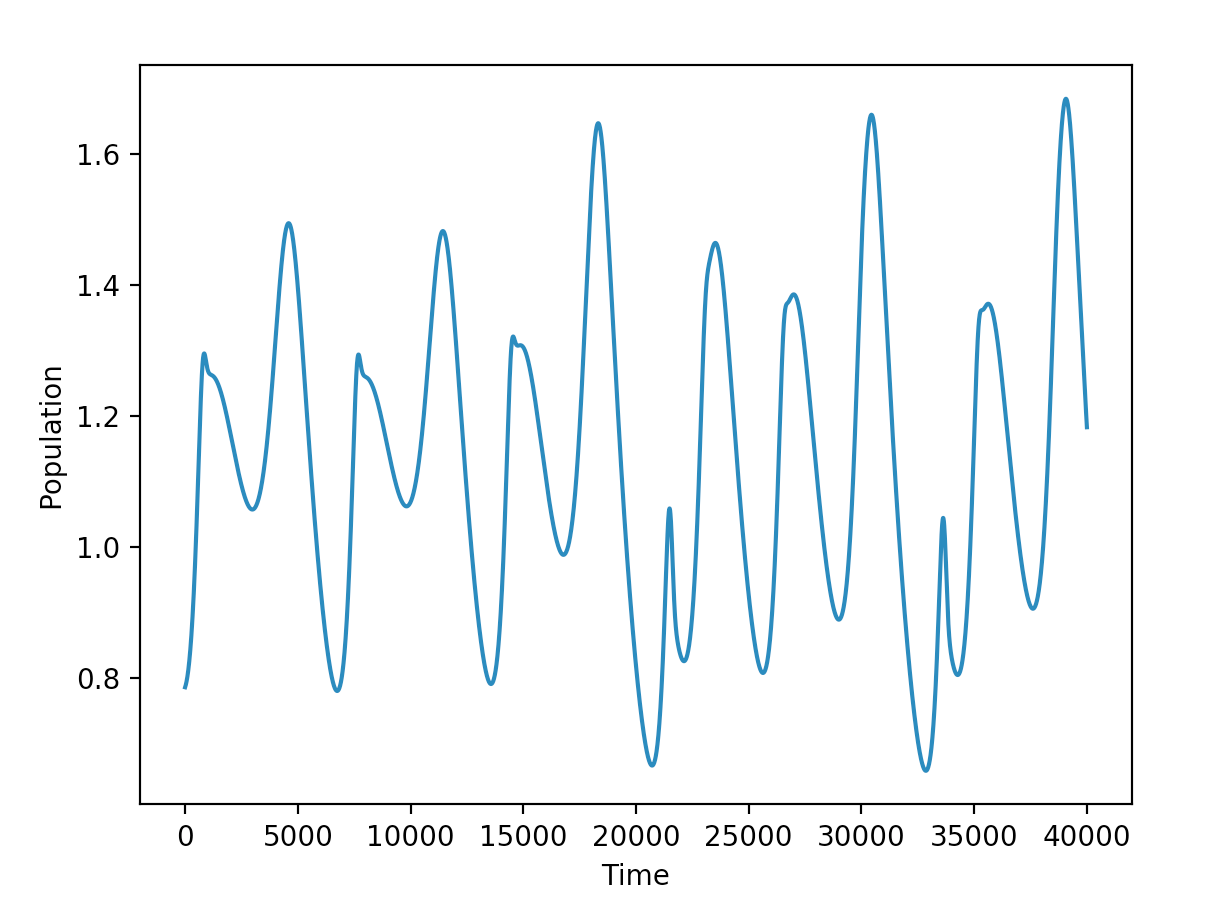
\includegraphics[width=0.5\textwidth]{dataspikes.png}}
   \caption{\label{ref_label_overall}Time series showing spikes at irregular intervals and magnitudes. Notice that even spikes of similar shape return in a slightly altered form. This type of series may be best understood by networks containing LSTM cells.}
\end{figure} 

\begin{table}
\caption{Class Distribution of Data Sets}
\setlength{\tabcolsep}{5mm} % separator between columns
\def\arraystretch{1.25} % vertical stretch factor
\centering

  \begin{tabular}{|c|c|c|c|c|c|}
	\hline
     & \textbf{\textit{D}} &  \textbf{\textit{D\textsubscript{N}}} &  \textbf{\textit{D\textsubscript{3}}} &  \textbf{\textit{D\textsubscript{4}}} &  \textbf{\textit{D\textsubscript{5}}}\\ \hline
   \textbf{0} & 0.34 & 0.44 & 0.45 & 0.24 & 0.80\\ \hline
   \textbf{1} & 0.34 & 0.45 & 0.55 & 0.76 & 0.04\\ \hline
   \textbf{2} & 0.05 & 0.11 &  &  & 0.02\\ \hline
   \textbf{3} & 0.06 &  &  &  & 0.14\\ \hline
   \textbf{4} & 0.11 &  &  &  & \\ \hline
   \textbf{5} & 0.03 &  &  &  & \\ \hline
   \textbf{6} & 0.02 &  &  &  & \\ \hline
   \textbf{7} & 0.05 &  &  &  & \\ \hline
  \end{tabular}
\end{table}

%\addtolength{\textheight}{-12cm}   % This command serves to balance the column lengths
                                  % on the last page of the document manually. It shortens
                                  % the textheight of the last page by a suitable amount.
                                  % This command does not take effect until the next page
                                  % so it should come on the page before the last. Make
                                  % sure that you do not shorten the textheight too much.

%%%%%%%%%%%%%%%%%%%%%%%%%%%%%%%%%%%%%%%%%%%%%%%%%%%%%%%%%%%%%%%%%%%%%%%%%%%%%%%%
\section{CONCLUSIONS}
	The presence of chaos in the natural and unnatural world has sparked the interest of many of the greatest minds of our time. Its seemingly random, yet deterministic nature has been found throughout our world and others and has been shown to help explain many difficult phenomena. In the natural world the presence of chaos in ecological systems, particular in their cycles of populations, has allowed for further in depth analysis of the world around us. 

	The precise aspect of chaos that draws many to it makes it puzzling to those who ponder it. It's difficulty to characterize and predict has challenged many researchers. Using different Machine Learning algorithms, this report has strove to gain an insight into chaos, showing that for the specific task of topological inference in ecologic networks, complex models such as a CNN-LSTM can better capture the essence of the data. This finding enlightens future researchers by giving a sturdier understanding of the characteristics and tools needed to analyze chaotic populations. 
    
    It is suggested that future research focus on the development of (1) a higher quality dataset with more even class distributions, and (2) classification models more capable of understanding the data. Also of interest would be (3) the determination of whether or not chaotic time series produced by the models used above are indeed classifiable. 
    
%%%%%%%%%%%%%%%%%%%%%%%%%%%%%%%%%%%%%%%%%%%%%%%%%%%%%%%%%%%%%%%%%%%%%%%%%%%%%%%%
\section{ACKNOWLEDGMENTS}
		Many thanks are owed to those individuals who took time to aid in the completion of this report. Frederic Guichard, the supervisor of this study, provided endless insight into the world of chaos and dynamical systems which I had not had any previous training in. Professor Guichard aided in narrowing the scope of the project to a manageable size, and pointed research in a helpful direction when roadblocks were met. I would like to thank also, and perhaps strangely, my trumpet teacher Russel DeVuyst for leading by example and teaching lessons that could be carried far outside of the practice room, showing that age does not need to diminish curiosity and enthusiasm, and for understanding that my interests spanned many disciplines. To my family are owed the greatest thanks, for their support and love, for their ability to listen to rants filled with mathematical terminology and endless requests to look at strange attractors. Lastly, I would like to the 5b's Bakery in Concrete, Washington for providing me with a space to camp out for many hours on end to complete the report, and for their endless coffee. 

%%%%%%%%%%%%%%%%%%%%%%%%%%%%%%%%%%%%%%%%%%%%%%%%%%%%%%%%%%%%%%%%%%%%%%%%%%%%%%%%
\begin{thebibliography}{99}

\bibitem{c1}Decai Li, Min Han and Jun Wang. “Chaotic Time Series Prediction Based on a Novel Robust Echo State Network.” IEEE Transactions on Neural Networks and Learning Systems 23: 787-799. (2012).

\bibitem{c2} Thomas G. Dietterich. "Machine Learning for Sequential Data: A Review". Structural, Syntactic, and Statistical Pattern Recognition, Lecture Notes in Computer Science, vol 2396. (2002).

\bibitem{c3} Edward N Lorenz. "The Essence of Chaos". University of Washington Press. (1993).

\bibitem{c4} Gregor F. Fussmann and Gerd Heber. “Food web complexity and chaotic population dynamics.” (2002).

\bibitem{c5} Luis J. Gilarranz, Alan Hastings, and Jordi Bascompte. "Inferring topology from dynamics in spatial networks". Theor Ecol 8: 15. https://doi.org/10.1007/s12080-014-0231-y. (2015).

\bibitem{c6} Alex Graves and Jurgen Schmidhuber. "Framewise phoneme classification with bidirectional LSTM and other neural network architectures". Neural Networks, 18:602–610. (2005).

\bibitem{c7} Aaron Klebanoff and Alan Hastings. "Chaos in one-predator, two-prey models: general results from bifurcation theory." A. J. Math. Biol. 32: 427. https://doi.org/10.1007/BF00160167. (1994).

\bibitem{c8}Aaron Klebanoff and Alan Hastings (1994). "Chaos in three species food chains". J. Math. Biol. 32, 427–451. (1994).

\bibitem{c9} Jacques Maquet and Christophe Letellier. "Global models from the Canadian lynx cycles as a direct evidence for chaos in real ecosystems".  L.A. J. Math. Biol. 55: 21. https://doi.org/10.1007/s00285-007-0075-9. (2007)

\bibitem{c10} Marc Barthelemy, Jean-Pierre Nadal, and Henri Berestycki. PNAS 107 (17) 7629-7634;https://doi.org/10.1073/pnas.0910259107. 

\bibitem{c12} Mohammad Norouzi, Mani Ranjbar, and Greg Mori. "Stacks of convolutional Restricted Boltzmann Machines for shift-invariant feature learning". IEEE Conference on Computer Vision and Pattern Recognition. (2009).

\bibitem{c12} Paola Vera-Licona and Reinhard Laubenbacher. "Inference of ecological interaction networks". Annales Botanici Fennici, 45: 459-464. (2008).

\bibitem{c13} Athanasios Voulodimos, Nikolaos Doulamis, Anastasios Doulamis, and Eftychios Protopapadakis, “Deep Learning for Computer Vision: A Brief Review". Computational Intelligence and Neuroscience, vol. 2018, Article ID 7068349. https://doi.org/10.1155/2018/7068349. (2018).

\bibitem{c14} William M. Schaffer and Mark Kot. "Do Strange Attractors Govern Ecological Systems?". BioScience, Volume 35, Issue 6, 342–350, https://doi.org/10.2307/1309902. (1985).

\bibitem{c15} Zachary C. Lipton, John Berkowitz, and Charles Elkan. "A critical review of recurrent neural networks for sequence learning". arXiv preprint arXiv:1506.00019. (2015).
\end{thebibliography}

\end{document}